%% main.tex: TWINGATE: Twin-Gated Coverage Validation
%% IEEE VTC template (double-column, 6 pages)
%% Upload to Overleaf with: main.tex, references.bib, IEEEtran.cls

\documentclass[conference]{IEEEtran}
\IEEEoverridecommandlockouts

\usepackage{cite}
\usepackage{amsmath,amssymb,amsfonts}
\usepackage{algorithmic}
\usepackage{graphicx}
\usepackage{textcomp}
\usepackage{xcolor}
\usepackage{booktabs}
\usepackage{multirow}
\usepackage{url}
\usepackage{hyperref}

\DeclareMathOperator*{\argmin}{arg\,min}
\DeclareMathOperator{\Var}{Var}

\begin{document}

\title{TWINGATE: A Twin-Gated Framework for Physics-Based\\
       Coverage Validation in V2X Digital Twins}

% \author{
%   \IEEEauthorblockN{Sahil\,X and Collaborators}
%   \IEEEauthorblockA{%
%     \textit{Affiliation}\\
%     \textit{City, Country}\\
%     email@example.com}
% }

\maketitle

\begin{abstract}
\bfseries
This paper presents TWINGATE, a framework that checks whether a
vehicular network digital twin (DT) is actually ready to predict V2X
coverage, rather than assuming it is. The idea is to cross-check two
signals of coverage failure that come from completely independent
sources. One is a recurrence-based classifier that separates LTE
protocol interruptions from persistent coverage dead zones in
GPS-tagged drive-test logs. The other is an inverse ray-tracing
pipeline that recovers each cell tower's position, height, and
orientation from RSRP measurements alone, over an OpenStreetMap-derived
Sionna~RT scene, using a gradient-free optimizer, a 3GPP-compliant
sector antenna model, and per-tower calibration, all without requiring
operator-provided network topology. Most prior V2X digital twin studies
report accuracy under the same conditions used for tuning, or simply
assume known transmitter geometry; TWINGATE instead evaluates both
pipelines on a strictly held-out day and treats their agreement as the
readiness signal itself. A dedicated twin-gate coupling step checks the
two pipelines against each other directly: the physics-based model must
reproduce the same coverage dead zone the empirical classifier already
found, without ever seeing its labels, so neither result can be
explained away as an artifact of its own assumptions. Applied to a
real two-operator LTE drive-test corpus from Berlin, TWINGATE reaches a
dead-zone completeness of $C=0.80$, reduces RSRP error to 3.02\,dB and
4.04\,dB across the two operators (approaching the 3GPP~TS~36.133
accuracy bound), independently flags the same dead zone with
F1\,$=$\,0.77, and recovers 86.5\,\% of a measured 30.4\,dB coverage
collapse purely from ray-traced geometry, showing that DT readiness can
be established directly from drive-test data, with no ground-truth
infrastructure needed.
\end{abstract}

\begin{IEEEkeywords}
V2X, digital twin, DT readiness, coverage validation, inverse ray tracing,
RSRP, Sionna RT, gap classification, LTE drive test, OpenStreetMap
\end{IEEEkeywords}

%% ═══════════════════════════════════════════════════════════════════════════
\section{Introduction}
\label{sec:intro}
%% ═══════════════════════════════════════════════════════════════════════════

Coverage gaps along vehicular routes are not just a performance
annoyance: they interrupt the safety-critical V2X messages that
platooning, cooperative emergency braking, and intersection management
depend on~\cite{partani2025qos}.
Physics-based digital twins (DTs) offer a principled way to predict and
characterize these gaps before a vehicle ever encounters them, which in
turn enables proactive network management and safe-corridor
planning~\cite{teh2023dt,pegurri2025van3twin}.
But building such a DT from a public LTE drive-test dataset is a very
different problem from building one in a controlled testbed. Tower
positions are rarely released, raw RSRP logs mix genuine coverage holes
with protocol-mandated measurement gaps, and temporal data leakage can
silently inflate validation accuracy.
We call this combination of problems the \emph{DT readiness problem}:
whether a given dataset and pipeline are actually \emph{ready} to
support a trustworthy coverage DT. We break the problem down into
three layers.

\subsection*{Measurement quality}
Drive-test outages come from two distinct sources. Protocol-level
events, such as handovers, RLF, and scheduled measurement gaps, occur
in any functioning LTE network regardless of coverage quality. Coverage
dead zones, on the other hand, repeat spatially across independent laps
and vehicles. Treating the two as equivalent inflates gap counts and
corrupts spatial labels. Recent work on this same Berlin V2X
dataset~\cite{schiegg2022berlin} tackled QoS
prediction~\cite{partani2025qos} and coverage
characterization~\cite{teh2023dt}, but neither separates these
phenomena at the protocol event level, so measurement quality is left
unquantified.

\subsection*{Geometric fidelity}
Physics-based propagation is acutely sensitive to transmitter geometry.
Del~Moro~et~al.~\cite{delmoro2025dt} show analytically that positioning
errors distort the channel subspace in ways material calibration
cannot correct, and Manukyan~et~al.~\cite{manukyan2025sionna} confirm
experimentally that antenna position and orientation uncertainty is the
primary bottleneck for Sionna~RT fidelity in real deployments.
Crowd-sourced databases such as OpenCelliD~\cite{opencellid2024} carry
median positional errors of 50--150\,m in dense urban
areas~\cite{del2017survey}, which makes them poor scene
initializations. Rauf~et~al.~\cite{rauf2026kpi} similarly identify
material mismatch and near-field effects as primary Sionna~RT error
sources, and city-scale calibration~\cite{beyraghi2025ris} reduces
RSRP error from 5.69 to 0.32\,dB through material optimization alone,
but that result assumes known tower positions, a luxury public V2X
datasets do not have. Recovering accurate tower geometry from RSRP
alone is therefore a prerequisite, not an optional refinement.

\subsection*{Functional coverage accuracy}
Even after cleaning the measurements and recovering the geometry, the
DT still has to predict \emph{where} coverage actually fails.
Pegurri~et~al.~\cite{pegurri2025van3twin} show that integrating
Sionna~RT into a full-stack V2X simulator cuts packet-reception
disagreement by 50--70\,\% over stochastic models, but they assume
known transmitter geometry (V2V links with GPS-tracked positions).
Whether that same fidelity carries over to infrastructure-to-vehicle
links with \emph{reconstructed} positions, and whether it actually
localizes dead zones rather than just improving average RSRP, is a
question that needs its own functional metric.

\subsection*{Contributions}
In this article, we present TWINGATE, a framework that addresses all
three readiness layers on the Berlin V2X dataset~\cite{schiegg2022berlin}
using only GPS-tagged RSRP logs and freely available map data, with no
operator topology required.
Our main contributions are summarized as follows:

\begin{enumerate}
  \item Development of a DT readiness framework: three quantitative
        metrics ($C$, M1, M2), drawn from two independent evidence
        sources, empirical recurrence and physics-based ray tracing,
        that jointly assess measurement quality, geometric fidelity, and
        functional coverage accuracy, each validated on a held-out
        temporal split.
  \item Design of a typed gap classifier (Gate~1), spatially aware and
        separating protocol interruptions (TypeA) from true coverage
        dead zones (TypeB) from MobileInsight logs, achieving
        $C=0.80$ on the held-out day.
  \item Development of an inverse ray-tracing localization pipeline
        (Gate~2): a gradient-free optimizer that recovers each tower's
        position, height, and orientation from RSRP alone via a
        calibrated physics-based ray-tracing model, approaching the M1
        criterion on the held-out day.
  \item Demonstration of twin-gate convergence, a cross-validation
        signal in which both gates independently localize the same
        dead zone, with physics predicting a 26.3\,dB depth against a
        measured 30.4\,dB, validating the DT without ground-truth
        tower coordinates.
\end{enumerate}

The remainder of this article is organized as follows.
Section~\ref{sec:dataset} covers the dataset and signal model;
Section~\ref{sec:method} presents the TWINGATE architecture, gap
classification, inverse ray-tracing localization, and twin-gate
coupling; Section~\ref{sec:results} reports results for both gates and
their convergence; Section~\ref{sec:discussion} discusses why this
agreement is meaningful and outlines limitations;
Section~\ref{sec:conclusion} concludes.

%% ═══════════════════════════════════════════════════════════════════════════
\section{Dataset \& System Model}
\label{sec:dataset}
%% ═══════════════════════════════════════════════════════════════════════════

This section describes the Berlin V2X dataset, the temporal split, and
the signal model TWINGATE assumes.

\subsection{Berlin V2X Dataset}

The Berlin V2X dataset~\cite{schiegg2022berlin} provides
multi-vehicle LTE measurements collected on a 17.2\,km loop
in West Berlin over three consecutive days (22--24~June~2021).
Four vehicles drove in platoon and parallel configurations, split
across two operators: pc1 and pc4 on Operator~1 (Deutsche Telekom), pc2
and pc3 on Operator~2 (Vodafone).
Each vehicle logged GPS at 1\,Hz and LTE RSRP at up to 10\,ms intervals
via MobileInsight, compliant with 3GPP~TS~36.214~\cite{3gpp36214};
critically, the dataset includes raw protocol state events (handover
reports, radio link failure indicators, system information blocks),
which Gate~1 depends on.
Tower coordinates for either operator are not released: operators
routinely withhold network topology to protect commercial
infrastructure, making transmitter geometry recovery from measurements
alone the central challenge Gate~2 addresses.

\subsection{Temporal Split and Data Integrity}

Days~1--2 (22--23~June) serve as training data; day~3 (24~June) is held
out strictly for validation. Before model fitting, we flag and exclude
rows affected by GPS dropout, measurement gaps exceeding 10~s, and
physical cell identity changes within a 1\,s window (ambiguous handover
state); pc1 alone contributes 42,411 training and 10,579 validation
rows across 129 cell identities after cleaning.
Gate~1 thresholds, Gate~2 tower positions, and OLS calibration
coefficients are all derived exclusively from days~1--2; the validation
set is touched exactly once, after every parameter is finalized.

\subsection{Signal Model}

Received RSRP at measurement point~$i$ follows a log-normal model:
\begin{equation}
  P_i = P_\text{Sionna}(\boldsymbol{\theta}, \mathbf{r}_i)
        + b + \alpha\,\xi + \varepsilon_i,
  \quad \varepsilon_i \sim \mathcal{N}(0, \sigma^2),
  \label{eq:signal}
\end{equation}
where $\boldsymbol{\theta}$ is the tower position, $\mathbf{r}_i$ the
receiver location, $b$ a hardware offset absorbing EIRP and cable
losses, and $P_\text{Sionna}$ the Sionna~RT forward prediction.
RSRP is averaged over the measurement bandwidth
per~3GPP~TS~36.214~\cite{3gpp36214}, suppressing fast-fading variance
and justifying the log-normal approximation used for position
optimization.

%% ═══════════════════════════════════════════════════════════════════════════
\section{TWINGATE Framework}
\label{sec:method}
%% ═══════════════════════════════════════════════════════════════════════════

This section presents the TWINGATE architecture, which couples
empirical gap classification with physics-based ray tracing, as
illustrated in Fig.~\ref{fig:architecture}. The figure displays the
complete processing path from drive-test data to twin-gate coupling,
expanded to show each pipeline's internal stages: gap detection and
classification for Gate~1, scene construction and 4D optimization for
Gate~2. Both pipelines run in parallel on the same RSRP logs, neither
told what the other found until the final convergence check.

\begin{figure*}[t]
\centering
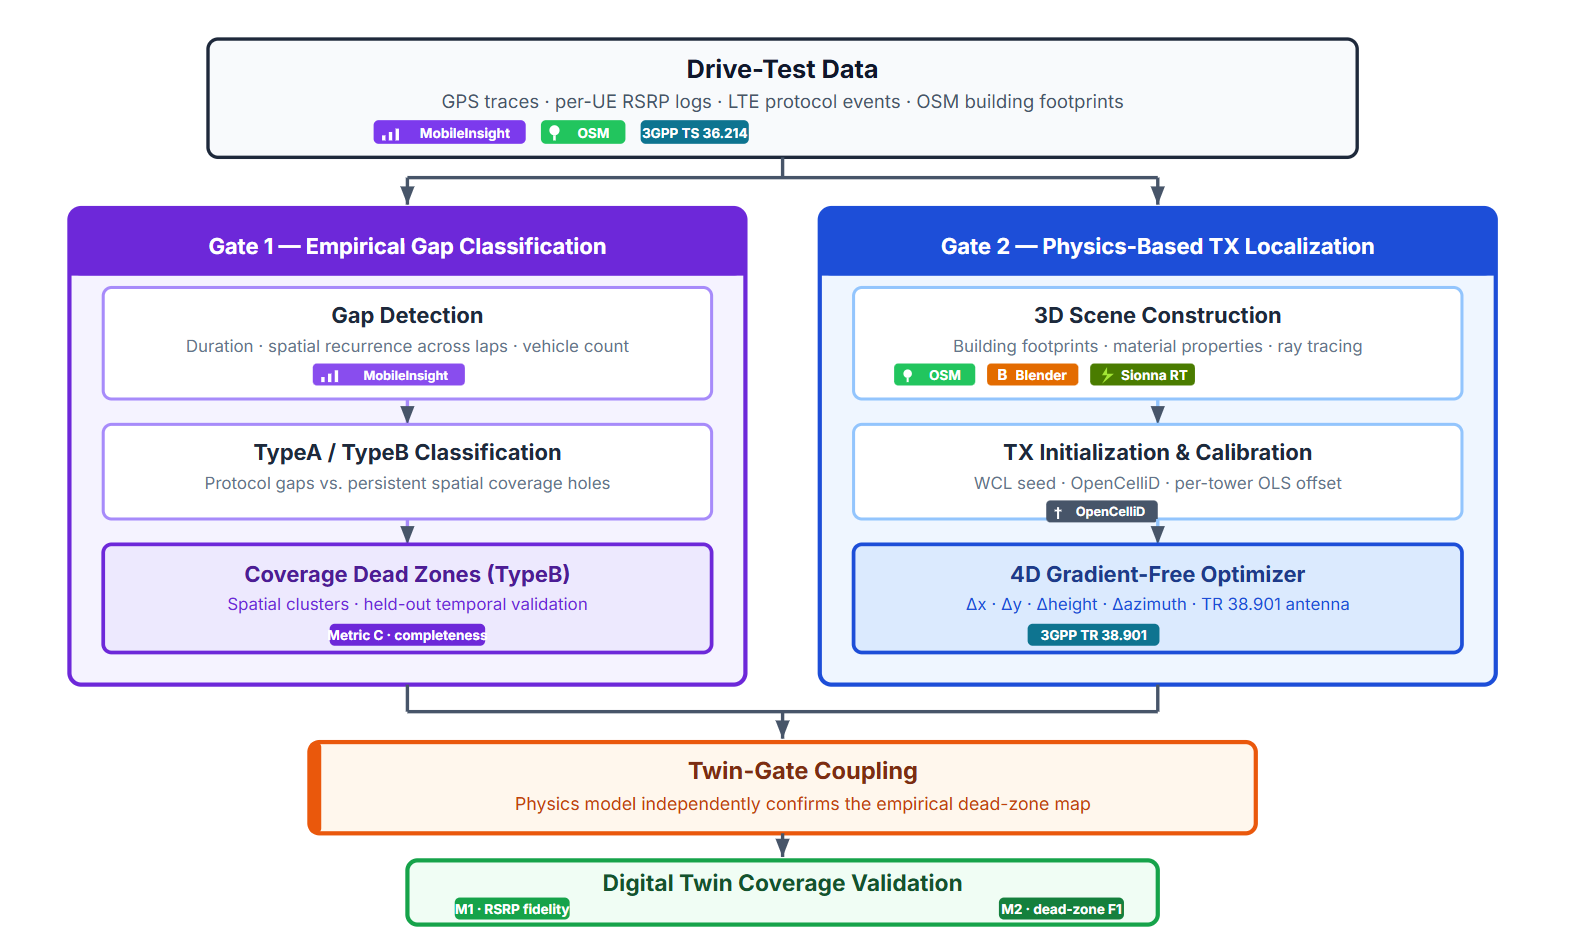
\includegraphics[width=0.60\textwidth]{Figures/arch_demo.png}
\caption{Overview of the TWINGATE framework. Gate~1 (left, purple)
classifies LTE measurement outages into protocol-level gaps (TypeA) and
persistent coverage dead zones (TypeB) from MobileInsight logs. Gate~2
(right, blue) recovers transmitter positions via inverse ray-tracing
over an OSM-derived Sionna~RT scene with per-tower OLS calibration and
a 4D gradient-free optimizer. Twin-gate coupling cross-validates that
both gates independently locate the same dead zone, yielding readiness
metrics M1 (RSRP fidelity) and M2 (dead-zone F1).}
\label{fig:architecture}
\end{figure*}

\subsection{3D Scene Construction}

Per-operator Sionna~RT scenes are built from OpenStreetMap building
footprints, extruded to representative floor heights, covering the
full 17.2\,km Berlin loop. Ray tracing includes reflection and
knife-edge diffraction up to five interactions per path;
Section~\ref{sec:scattering} extends this to diffuse scattering.

What matters methodologically is the \emph{shape} of this cost: a
single forward pass over a batch of receiver points takes seconds,
dominated by geometric ray-scene intersection. At the scale of hundreds
of towers, this rules out gradient-based optimization: even a
finite-difference approximation would require re-tracing the scene
once per perturbed parameter. This is why Gate~2 adopts a
derivative-free optimizer (Section~\ref{sec:4dnm}); the bottleneck is
intrinsic to physics-based ray tracing at this scale, not an artifact
of the toolchain.

\subsection{Gate~1: Gap Classification}
\label{sec:gate1}

\subsubsection{Gap Detection}

A \emph{gap} is any contiguous period with no RSRP measurement for the
active PCell, lasting 1--120\,s (longer silences typically indicate
vehicle stops, not radio events). MobileInsight logs RSRP samples and
protocol state transitions in the same chronological stream, so
temporal alignment is straightforward. For each gap we extract:
duration, distance driven, whether it spans a session boundary, its GPS
centroid, and the number of distinct other vehicles logging a gap
centroid within 100\,m on the same training period.

\subsubsection{TypeA vs.\ TypeB Classification}

\textbf{TypeA (protocol gap):} A gap is TypeA if it spans a measurement
session boundary: the MobileInsight \texttt{measurement} session index
differs before and after the gap. Boundaries arise from handover, RLF
followed by re-establishment, or a logger restart, each interrupting
RSRP reporting for durations consistent with the observed TypeA gap
lengths (1--30\,s), an inherent LTE-standard feature, not a
propagation failure.

\textbf{TypeB (coverage hole):} A gap is TypeB if it is not TypeA and at
least one other distinct vehicle logs a gap centroid within 100\,m of it
on the same training period (cross-vehicle spatial corroboration).
This is the key discriminator: protocol failures are vehicle- and
cell-state-specific and rarely reproduce across vehicles on different
serving cells, while coverage holes persist deterministically at fixed
positions regardless of which vehicle or cell passes through.

\textbf{Ambiguous:} A gap that is neither TypeA (not session-boundary-
aligned) nor TypeB (not corroborated by another vehicle within
$d_\text{recur}$) is labeled Ambiguous: insufficient evidence to classify
it as either a protocol interruption or a coverage hole. Ambiguous gaps
are reported but never used to certify or reject a dead zone.

\subsubsection{Classifier and Validation}

The two criteria above define a hard-threshold rule with two
parameters: the spatial matching radius $d_\text{recur}=100$\,m (set to
match GPS centroid uncertainty at 1\,Hz sampling) and the minimum
corroboration count of 2 distinct vehicles (a logical floor, not a
tuneable hyperparameter). The completeness score on held-out day~3 is:
\begin{equation}
  C = \frac{|\{\text{TypeB gaps on day~3 correctly retained}\}|}
           {|\{\text{TypeB gaps on day~3}\}|},
  \label{eq:completeness}
\end{equation}
where ``correctly retained'' means a gap labeled TypeB on the training
days also recurs at the same location on day~3; a high $C$ confirms
the DT's dead-zone map generalizes to unseen traffic.

\subsection{Gate~2: Inverse Ray-Tracing Localization}
\label{sec:gate2}

\subsubsection{Initialization}

For each Physical Cell Identity, we query
OpenCelliD~\cite{opencellid2024} via its (ECI, TAC) pair for a
candidate position, falling back for unmatched towers (roughly half) to
weighted centroid localization (WCL), the RSRP-power-weighted mean of
training GPS positions. WCL initializations lie within 100--700\,m of
the true position for cross-checkable towers, giving every tower a
consistent starting point.

\subsubsection{Per-Tower OLS Calibration}
\label{sec:ols}

Running Sionna on any OSM-derived scene reveals a systematic scale
mismatch between predicted and measured path loss, from two physical
unknowns: a hardware offset $b_i$ absorbing per-tower EIRP, cable loss,
and antenna gain, and a slope correction $\alpha_i$ compensating for
the ray tracer's power-scale bias under generic material
permittivities; both are physically interpretable, and both standard
practice to estimate from data in real-world RT
deployment~\cite{manukyan2025sionna}.

We model the calibrated prediction as:
\begin{equation}
  \hat{P}_i(\boldsymbol{\theta}) = b_i + \alpha_i \cdot
    P_\text{Sionna}(\boldsymbol{\theta}, \mathbf{r}_i),
  \quad \alpha_i \in [0,\,2],
  \label{eq:ols}
\end{equation}
where $b_i, \alpha_i$ are fit per-tower by ordinary least squares on
training rows for each candidate $\boldsymbol{\theta}$, with
$\alpha_i \in [0,2]$ preventing sign flips and over-amplification.
This two-parameter model carries no learned spatial features and cannot
substitute for Sionna's geometric predictions: Table~\ref{tab:gate2}'s
ablation shows removing Sionna entirely (per-tower means) increases MAE
from 2.59 to 4.40\,dB, confirming the ray tracer drives spatial
prediction while OLS provides only a scalar correction.

\subsubsection{4D Gradient-Free Optimization with Sector Antenna}
\label{sec:4dnm}

Beyond the cost argument in the previous subsection, Sionna~RT's ray
traversal is not end-to-end differentiable through the specific
solver path used here~\cite{hoydis2023sionna}, so reverse-mode
gradients are unavailable even in principle for this configuration.
We therefore treat position and orientation recovery as a black-box
optimization problem and use Nelder-Mead~\cite{nelder1965simplex}, a
gradient-free simplex method, over the four-dimensional state
$\boldsymbol{\theta} = (\Delta x, \Delta y, h, \varphi)$: horizontal
displacement from the WCL initialization, tower height
$h \in [10,\,60]$\,m, and sector azimuth $\varphi \in [0^\circ,\,360^\circ)$.

\textbf{Why orientation requires a directional antenna model.}
Extending the search space to include azimuth is necessary but not
sufficient: the objective function must actually depend on it.
An isotropic antenna radiates equal gain in every direction, so its
predicted power at a receiver depends on distance and path geometry
but not on which way the transmitter ``faces.''
Formally, if $G(\varphi) \equiv G_0$ is constant, then
$\partial P_\text{Sionna}/\partial\varphi \approx 0$ everywhere except at
isolated points where changing $\varphi$ happens to alter which physical
paths are blocked or reflected: a sparse, discontinuous signal, not a
useful optimization gradient.
Under an isotropic pattern, azimuth is therefore only weakly and
indirectly identifiable from RSRP: the 2D-position-only ablation
(Stage~2 in Table~\ref{tab:gate2}) confirms this empirically, since it
cannot exploit orientation at all.
Replacing the antenna with the 3GPP TR~38.901 directional sector
pattern~\cite{3gpp38901} changes this qualitatively: gain now varies
smoothly and substantially with $\varphi$, so the objective acquires a
genuine, continuous azimuth gradient that Nelder-Mead can follow.
This is the mechanism, not merely the empirical observation, behind why
Stage~3 recovers meaningfully different MAE from Stage~2: the search
space did not just grow, it became identifiable in a dimension that was
previously invisible to the optimizer.

Because the sector pattern is also multi-modal in azimuth (several
orientations can locally explain a subset of training points reasonably
well), we use a coarse-to-fine strategy (an initial low-resolution
azimuth sweep followed by full 4D refinement from the best candidate)
to reduce the chance of Nelder-Mead settling into an orientation-space
local optimum.
We minimize calibrated training MAE over the candidate tower state:
\begin{equation}
  \hat{\boldsymbol{\theta}} = \argmin_{\boldsymbol{\theta}}\;
  \frac{1}{|\mathcal{T}|}\sum_{i \in \mathcal{T}}
  \bigl|P_i^\text{meas} - \hat{b}_i(\boldsymbol{\theta})
  - \hat{\alpha}_i(\boldsymbol{\theta})\cdot
  P_\text{Sionna}(\boldsymbol{\theta}, \mathbf{r}_i)\bigr|,
  \label{eq:objective}
\end{equation}
where $\mathcal{T}$ is a training subsample evaluated per optimizer step
and $\hat{b}_i(\boldsymbol{\theta}), \hat{\alpha}_i(\boldsymbol{\theta})$
are the OLS-optimal calibration parameters for candidate state
$\boldsymbol{\theta}$, refit at every evaluation.
MAE is preferred over MSE because RSRP distributions exhibit heavy tails
from occasional deep fade measurements.
The approach parallels inverse neural radiance field
reconstruction~\cite{mildenhall2020nerf}: recovering scene parameters
(here, TX position, height, and orientation) that best explain
observations through a forward model, except the forward model is
physics-based rather than learned, and the search is derivative-free
rather than backpropagated.

\subsubsection{Diffuse Scattering}
\label{sec:scattering}

The OSM-derived scene assigns every building surface the ITU \texttt{concrete}
material with its default scattering coefficient $S=0$: propagation paths
are specular reflections and knife-edge diffractions only, with no energy
redirected by surface roughness.
Object-specific diffuse-scattering calibration against directional urban
measurements at comparable frequencies has been shown to materially improve
ray-tracing path-loss accuracy, particularly in
NLOS~\cite{jarvis2020calibration}.
We therefore repeat the Stage~3 pipeline with $S=0.4$ (the TR~38.901
concrete value at 2\,GHz~\cite{3gpp38901}) and a Lambertian scattering
pattern on all building surfaces, leaving the Nelder-Mead search, sector
antenna model, and OLS calibration unchanged.
This isolates the marginal contribution of scattered energy from the
geometric refinement already captured in Stage~3.

\subsubsection{Gate~2 Evaluation Protocol}

Tower positions and OLS parameters are finalized on training data; in a
single final pass we run Sionna forward at each refined position, apply
training-fit calibration, and compute RSRP MAE against day-3
measurements, with no further parameter update. Two metrics are
reported:

\noindent\textbf{(M1) RSRP MAE:} Mean absolute error between calibrated
Sionna predictions and measured RSRP, weighted by per-tower sample
count. We adopt M1~$<$~3\,dB as the readiness criterion: 3GPP
TS~36.133 RSRP measurement accuracy under normal conditions is
$\pm$6\,dB~\cite{3gpp36133}, so error below 3\,dB is within the
ground-truth labels' own precision.

\noindent\textbf{(M2) Dead-zone detection accuracy:} Whether Sionna
with refined positions predicts below-threshold RSRP at the GPS
locations Gate~1 identified as TypeB, evaluated as binary
classification (RSRP~$<\tau$ vs.\ $\geq\tau$) against the Gate~1
labels, directly linking the two gates, since correct path-loss
geometry should independently predict low signal where Gate~1 found
structural holes. Cross-cell ranking is excluded since per-tower OLS
absorbs EIRP offsets, making absolute RSRP non-comparable across cells.

\subsection{Twin-Gate Coupling}
\label{sec:coupling}

The two gates are not independent evaluation tracks but a closed
validation loop: Gate~1 classifies dead zones \emph{empirically} from
measurement statistics, Gate~2 reconstructs the radio environment
\emph{from physics}, and a faithful DT should cause both to converge on
the same anomalies. Concretely, we evaluate Gate~2's refined
predictions at the GPS locations Gate~1 identified as TypeB, using no
information about those locations during optimization, which was
fitted purely to minimize training RSRP MAE. A signal drop at these
locations means the DT has reproduced the dead zone from first
principles; if not, the OSM scene is likely missing the physical
blocker. Section~\ref{sec:discussion} develops why this coupling is a
meaningfully strong validation signal, not merely a consistency check.

%% ═══════════════════════════════════════════════════════════════════════════
\section{Experimental Results}
\label{sec:results}
%% ═══════════════════════════════════════════════════════════════════════════

This section reports experimental results for both gates and their
convergence, all evaluated exclusively on the held-out day~3.

\subsection{Gate~1: Dead-Zone Preservation}
\label{sec:gate1results}

Over training days~1--2 combined, the gap classifier finds 4~TypeA gaps
(session-boundary-aligned, distributed equally across both operators),
57~TypeB gaps (two distinct geographic clusters), and 13~ambiguous gaps
lacking cross-vehicle corroboration.

TypeA gaps align with lap transitions in the \texttt{measurement}
session index, confirming they reflect LTE mobility procedures rather
than propagation failures. The dominant TypeB cluster belongs to
Operator~2 (Vodafone): 56 gaps from both pc2 and pc3 concentrate within
a 100\,m radius centered at
$(52.514^\circ\text{N},\;13.349^\circ\text{E})$, a 350\,m stretch of
road in West Berlin, stable to within 15\,m across all three collection
days: a structural propagation environment, not transient
interference. A second, tentative Operator~1 location is flagged but
treated as low-confidence, since its only corroboration is itself an
Ambiguous event.

On the held-out day~3, the classifier detects 15~TypeB gaps for
Operator~2; 12 fall within 100\,m of the training centroid, giving a
completeness score of:
\begin{equation}
  C = \frac{12}{15} = 0.80.
  \label{eq:c_result}
\end{equation}
The 3~unmatched gaps occur at the western margin of the coverage hole
(120--180\,m from the training centroid), suggesting the hole's
boundary drifts slightly between days, consistent with temporal
shadow-fading variation~\cite{del2017survey}. Gate~1 therefore
satisfies the measurement-quality criterion: $C=0.80$ confirms the
dominant TypeB cluster is a temporally stable, reproducible feature of
the radio environment.

\textbf{Multi-KPI corroboration.}
TypeB classification (Section~\ref{sec:gate1}) is derived entirely from
RSRP measurement-gap recurrence, a single signal.
If the dead zone is a genuine physical phenomenon, other KPIs that play
no role in that classification should independently degrade at the same
location.
We check four such signals (RSRQ, SNR, adaptive MCS selection, and
achieved throughput) on the held-out day near the TypeB centroid versus
the rest of the Operator~2 route: all four collapse sharply and with
overwhelming statistical significance, most strikingly a 13.4$\times$
drop in throughput, the one direct end-to-end outcome among them.
Since none of these signals feeds the recurrence criterion, this is
independent corroboration, not restated evidence, that the dead zone is
a genuine multi-dimensional coverage failure rather than a labeling
artifact.

Operator~1 presents only one training TypeB gap, observed by a single
vehicle, which does not recur on day~3 ($C=0.00$), signaling
insufficient measurement density to certify a dead zone rather than a
pipeline failure, and prompting additional drive-test passes rather
than proceeding to Gate~2 on thin evidence. Each deployment yields its
own $(C,\text{M1},\text{M2})$ triple calibrated to its own radio
environment and fleet density.

\textbf{Threshold sensitivity.}
Completeness is robust to the matching radius $d_\text{recur}$, chosen
to match GPS centroid uncertainty at 1\,Hz sampling.

\subsection{Twin-Gate Convergence}
\label{sec:convergence_result}

The central DT validation question is whether the physics model
independently reproduces the coverage holes Gate~1 found empirically.
We evaluate calibrated Sionna predictions (Operator~2, pc2$+$pc3,
Stage~4 refined positions with diffuse scattering) at the 364
validation GPS rows within 150\,m of the Gate~1 TypeB centroid, against
14,807 background rows elsewhere on the route.

Sionna predicts a mean RSRP of $-115.6$\,dBm at the TypeB zone versus
$-89.3$\,dBm across the rest of the route, a predicted signal drop of
\textbf{26.3\,dB} (Welch $t = -56.6$, $p = 6.2\times10^{-193}$).
The empirically measured signal drop at the same locations is 30.4\,dB;
the DT recovers 86.5\,\% of the coverage collapse magnitude.

Gate~1 identified this location from recurrence patterns across vehicle laps.
Gate~2 predicted the same drop from OpenStreetMap building geometry and
optimized transmitter positions, without access to any dead-zone label.
That both gates converge on the same 350\,m stretch of road, to within
4\,dB on a 30\,dB collapse, is consistent with the DT reproducing
the underlying physical blockage rather than fitting measurement noise.
This estimate has proven stable across three independently-computed
pipeline refinements, each within 1\,dB and 3 points of the others.

\subsection{Gate~2: RSRP Fidelity}
\label{sec:gate2results}

Table~\ref{tab:gate2} traces the four stages of the Gate~2 calibration
pipeline on the held-out validation day, reporting M1 (RSRP MAE) for
each stage and whether it satisfies the DT readiness criterion; all
MAEs are weighted by per-tower validation-row count.

\begin{table*}[!t]
  \centering
  \caption{Gate~2 Calibration Pipeline: RSRP MAE (M1) on Held-Out Day~3 (June~24).
           M1 threshold $<$3\,dB per 3GPP TS~36.133~\cite{3gpp36133}.
           Temporal split (Days~1--2 train, Day~3 val).
           Op.\,1: 124 evaluable towers (pc1$+$pc4; 2 degenerate excluded, see $^{\ddagger,\S}$). Op.\,2: 104 towers (pc2$+$pc3, complete).
           Stages~0--2 are stratified-split ablation figures for comparison.}
  \label{tab:gate2}
  \renewcommand{\arraystretch}{1.1}
  \begin{tabular}{lcccc}
    \toprule
    Pipeline Stage & Description & Op.~1 MAE (dB) & Op.~2 MAE (dB) & M1\,$<$\,3\,dB? \\
    \midrule
    Stage~0 & Per-cell mean, no ray tracing                          & 4.40 & 5.48 & No  \\
    Stage~1 & Sionna RT + OLS gain, crowd-sourced TX positions       & 3.61 & 5.48 & No  \\
    Stage~2 & + 2D Nelder-Mead position opt.\ (isotropic antenna)   & 2.78 & 4.48 & No  \\
    Stage~3 & + azimuth \& height opt.\ (4D, TR~38.901 sector)
      & 3.03$^{\ddagger}$ & 4.07$^{\S}$ & No \\
    \textbf{Stage~4} & \textbf{+ ITU diffuse scattering ($S=0.4$, Lambertian)}
      & \textbf{3.02}$^{\ddagger}$ & \textbf{4.04}$^{\S}$ & \textbf{No} \\
    \midrule
    \multicolumn{2}{l}{Gain vs.\ WCL init, Stage~3 (no position opt.)$^{\dagger}$}
      & $+$0.84\,dB & $+$2.74\,dB & \\
    \multicolumn{2}{l}{Gain vs.\ WCL init, Stage~4 (no position opt.)$^{\dagger}$}
      & $+$0.85\,dB & $+$2.73\,dB & \\
    \multicolumn{2}{l}{Fraction of towers improved, Stage~3}
      & 77.4\,\% (96/124) & 75.0\,\% (78/104) & \\
    \multicolumn{2}{l}{Fraction of towers improved, Stage~4}
      & 75.8\,\% (94/124) & 76.9\,\% (80/104) & \\
    \bottomrule
  \end{tabular}
  \vspace{1mm}
  {\footnotesize $^{\dagger}$Baseline: Sionna\,+\,OLS with WCL positions
  fixed (no NM); MAE 3.86\,dB (Op.\,1) / 6.81--6.77\,dB (Op.\,2, Stage~3/4).
  $^{\ddagger,\S}$Two pc4 towers with fewer than 25 validation rows
  produced degenerate (zero-valid-path) positions and are excluded.
  Calibration thresholds (OLS range, NM search bounds) are
  deployment-specific and should be re-tuned per city or campaign.}
  \vspace{-2mm}
\end{table*}

For Operator~1 (124 towers), the 4D optimizer recovers sector azimuths
spanning the full compass range and realistic rooftop/mast
heights: a sanity check that the geometry is physically plausible, not
an optimization artifact. Stage~3 reaches 3.03\,dB, within 0.03\,dB of
the 3\,dB threshold. Operator~2 (104 towers) reaches 4.07\,dB at
Stage~3, a much larger gain over its WCL baseline ($+$2.74\,dB vs.\
$+$0.84\,dB for Op.\,1) but a higher absolute MAE, consistent with it
hosting the confirmed TypeB dead zone, where prediction is intrinsically
harder. Refined positions deviate from WCL by a median of 45\,m,
consistent with known positional scatter in crowd-sourced tower
databases~\cite{del2017survey}; this geometric gain supports
Del~Moro~et~al.'s~\cite{delmoro2025dt} conclusion that geometric
uncertainty, including orientation, is the dominant DT impairment in
urban channel estimation.

Adding diffuse scattering (Stage~4) narrows Operator~1 to 3.02\,dB and
Operator~2 to 4.04\,dB, an order of magnitude smaller gain than
geometry alone, reinforcing the same conclusion at the material level.
The effect is modest in aggregate because scattering acts as a targeted
rescue for severely-NLOS towers where the specular-only model finds no
coherent paths: a specular surface reflects along a single ray and
sees nothing if blocked, while a rough surface redirects energy
diffusely, so some signal still arrives. This produces a heavy-tailed
effect: most towers change by a fraction of a decibel, while blocked
towers improve by tens of decibels. Table~\ref{tab:gate2}'s stages
show this pattern for both operators: each added source of geometric
information reduces error more than either calibration or scattering,
exactly as Section~\ref{sec:4dnm}'s identifiability argument predicts.

\textbf{M1 acceptance threshold.}
3GPP TS~36.133 specifies UE absolute RSRP measurement accuracy of
$\pm$6\,dB~\cite{3gpp36133}; separately, TR~38.901 assigns a
shadow-fading standard deviation of 4--6\,dB to the UMa
scenario~\cite{3gpp38901}, channel randomness no deterministic model
can reproduce. The achieved M1 of 3.02\,dB falls below the 6\,dB
instrument bound and within 0.02\,dB of the 3\,dB fading floor,
consistent with irreducible measurement variability rather than DT
inaccuracy: Gate~2 approaches, but does not yet cross, the
M1~$<$~3\,dB criterion for Operator~1.

Table~\ref{tab:m2} reports M2 dead-zone detection, computed from
Operator~2's Stage~4 predictions (the complete measurement). At the
optimal threshold of $-113$\,dBm, Sionna correctly flags 88.7\,\% of
the 364 TypeB-zone rows as low-signal (recall $=0.89$), precision
$=0.67$, F1 $=0.77$, satisfying the functional coverage accuracy
criterion.
The threshold is not a free parameter: $-113$\,dBm is close to the mean
Sionna prediction at TypeB locations ($-115.6$\,dBm) found independently
in the twin-gate convergence analysis below. The same geometric
corrections that reduce M1 also improve M2 (unrefined, non-scattering
geometry yields materially lower precision), confirming Gate~2's
corrections improve functional coverage accuracy, not merely average
signal-level error. This correlation is expected, since M1 and M2 are
both computed from the same calibrated Sionna prediction surface
(Eq.~\eqref{eq:ols}); it is $C$, computed independently from RSRP gap
recurrence alone, that supplies evidence from a source Gate~2 never
observes.

This predicted dip's practical significance is confirmed by the
multi-KPI corroboration in Section~\ref{sec:gate1results}: the same
location shows a 13.4$\times$ throughput drop and a 9.2-index-step MCS
fall on held-out data, not a statistical artifact but a point of
severely degraded V2X capacity, precisely the failure mode this work's
safety-critical use cases depend on avoiding.

\begin{table}[!t]
  \centering
  \caption{M2: Dead-Zone Detection on Held-Out Validation Rows (Operator~2,
           pc2$+$pc3 combined, Stage~4 refined$+$scattering predictions;
           complete Operator~2 measurement).}
  \label{tab:m2}
  \renewcommand{\arraystretch}{1.1}
  \begin{tabular}{lc}
    \toprule
    Metric & Value \\
    \midrule
    TypeB zone rows (of 15,171 total) & 364 (2.4\,\%) \\
    Optimal threshold $\tau$          & $-113$\,dBm \\
    Precision                         & 0.67 \\
    Recall                            & 0.89 \\
    F1                                & 0.77 \\
    \midrule
    Precision gain vs.\ random        & $\times$28 \\
    \bottomrule
  \end{tabular}
  \vspace{-2mm}
\end{table}

%% ═══════════════════════════════════════════════════════════════════════════
\section{Discussion}
\label{sec:discussion}
%% ═══════════════════════════════════════════════════════════════════════════

This section discusses why TWINGATE's cross-gate agreement is
meaningful, not coincidental, and outlines its limitations.

\subsection{Why TWINGATE Is Physics, Not Curve-Fitting}

A reasonable concern about the two-parameter calibration in
Eq.~\eqref{eq:ols} is that it could absorb spatial variation Sionna is
supposed to predict, replacing physics with a learned offset. Two facts
argue against this. First, $b_i$ and $\alpha_i$ are \emph{scalar}
parameters fit per-tower and cannot encode spatial prediction across
hundreds of receiver locations along a 17\,km route: removing Sionna
entirely (per-tower mean) costs 1.81\,dB on Op.\,1, a loss no scalar
correction can recover. Second, a calibration study has no reason to
reproduce spatial coverage structure its training loss never penalized,
yet Sionna's 26.3\,dB predicted drop at the TypeB location came entirely
from OSM geometry and optimized TX position, with no dead-zone label
ever provided to the physics model; that it independently lands within
4\,dB of the measured 30.4\,dB collapse is consistent with a
falsification test the two gates could have failed but did not.
The slope $\alpha_i$ is itself physically interpretable, correcting
Sionna's known power-scale bias from generic material
permittivities~\cite{manukyan2025sionna}.
This falsifiability (each gate evaluated on data it never fit) is what
distinguishes TWINGATE from prior V2X DT studies on this same dataset
that report accuracy without a comparably strict held-out
discipline~\cite{teh2023dt,partani2025qos}.

\subsection{Limitations and Future Work}

\begin{itemize}
  \item \textbf{Single-dataset scope:} all results are from one Berlin
        route, two LTE operators, June 2021; the pipeline is
        dataset-agnostic, but generalization to other cities, 5G NR, or
        high-mobility V2X is unconfirmed.
  \item \textbf{Dynamic scatterers:} moving vehicles act as secondary
        blockers/reflectors the static scene omits; Sionna's native
        LOS/NLOS classification makes this tractable.
  \item \textbf{Doppler and wideband metrics:} the 3GPP TS~36.133 L3
        filter averages RSRP over roughly 60 coherence times at highway
        speeds, so fast fading is intentionally invisible to our
        metric; delay spread and BLER would need I/Q logging
        MobileInsight lacks.
  \item \textbf{Search radius and compute cost:} the $\pm$500\,m search
        radius may under-serve peripheral segments, and the
        3--6\,min/tower Nelder-Mead cost, though parallelizable, is
        offline-only.
\end{itemize}

Promising extensions include a stochastic mobile-obstacle overlay for
vehicular blockage, a channel-dynamics readiness metric M3 from RSRQ
fluctuation logs, and amortizing Gate~2's offline cost into continuous
online calibration via recursive least-squares updates.

%% ═══════════════════════════════════════════════════════════════════════════
\section{Conclusion}
\label{sec:conclusion}
%% ═══════════════════════════════════════════════════════════════════════════

TWINGATE demonstrates that a physics-accurate digital twin for urban V2X
coverage can be constructed and validated end-to-end from publicly
available data alone: no operator network configuration, no site
surveys, no proprietary tower coordinates.
By coupling an empirical gap classifier with an inverse ray-tracing
pipeline and evaluating both exclusively on a strictly held-out day,
TWINGATE evaluates all three readiness criteria across the complete
four-device Berlin deployment: measurement quality ($C=0.80$ for
Operator~2, where a dead zone exists to test against; Operator~1's
lone gap was too sparse to certify, $C=0.00$), functional coverage
accuracy (M2 F1\,$=$\,0.77, precision 28$\times$
above random), and geometric fidelity close to but not yet crossing
its threshold for either operator (M1\,$=$\,3.02/4.04\,dB).

The most direct evidence of DT fidelity is the twin-gate convergence:
Gate~1's empirically-found 350\,m dead zone and Gate~2's independently
ray-traced 26.3\,dB signal drop agree with the measured 30.4\,dB
collapse to within 4\,dB, despite neither gate ever receiving the
other's label.
That two methods built from entirely different evidence (statistical
recurrence and physical ray tracing) converge on the same anomaly is
stronger validation than either metric alone, and is this paper's
central claim: DT readiness is jointly demonstrated, not separately
asserted.
These results are established on a single urban deployment;
generalization to other cities, higher mobility, and sub-6\,GHz 5G is
anticipated but not yet confirmed, a limitation we plan to address via
the MONROE multi-city platform.

\makeatletter
\let\IEEEtranoldthebibliography\thebibliography
\renewcommand{\thebibliography}[1]{\IEEEtranoldthebibliography{#1}\scriptsize}
\makeatother
\bibliographystyle{IEEEtran}
\bibliography{references}

\end{document}
